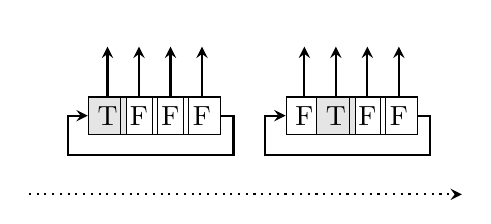
\begin{tikzpicture}
\tikzstyle{notused} = [rectangle, rounded corners , minimum width=3mm, minimum height=1mm,text centered, draw=black]
\tikzstyle{round}=[circle, minimum width=0mm,draw=black]
\tikzstyle{square} = [rectangle, minimum width=1mm, draw=black]
\tikzstyle{qraysquare} = [
rectangle, minimum width=1mm, draw=black, fill=gray!20]
\tikzstyle{empty}=[]

\usetikzlibrary{shapes.geometric, arrows}
\tikzstyle{arrow} = [thick,->,>=stealth]
\tikzstyle{dottarrow} = [thick, dotted,->,>=stealth]
\tikzstyle{noarrow}=[thick,-=,=stealth]

%node
\node (DA) [qraysquare] {T};
\node (DB) [square, right of =DA, xshift=-6mm] {F};
\node (DC) [square, right of =DB, xshift=-6mm] {F};
\node (DD) [square, right of =DC, xshift=-6mm] {F};

\node (DE) [square, right of =DD, xshift=3mm] {F};
\node (DF) [qraysquare, right of =DE, xshift=-6mm] {T};
\node (DG) [square, right of =DF, xshift=-6mm] {F};
\node (DH) [square, right of =DG, xshift=-6mm] {F};

%Epmty target nodes
\node (DAT) [empty, yshift=10mm]{};
\node (DBT) [empty, right of=DAT, xshift=-6mm]{};
\node (DCT) [empty, right of=DBT, xshift=-6mm]{};
\node (DDT) [empty, right of=DCT, xshift=-6mm]{};

\node (DET) [empty, right of=DDT, xshift=3mm]{};
\node (DFT) [empty, right of=DET, xshift=-6mm]{};
\node (DGT) [empty, right of=DFT, xshift=-6mm]{};
\node (DHT) [empty, right of=DGT, xshift=-6mm]{};

%lines to target node
\draw [arrow] (DA) -- (DAT);
\draw [arrow] (DB) -- (DBT);
\draw [arrow] (DC) -- (DCT);
\draw [arrow] (DD) -- (DDT);
\draw [arrow] (DD)  -- +(0.4,0) -- +(0.4,-0.5) -- (-0.5,-0.5) -+(-0.5,0.0) -- +(DA);

\draw [arrow] (DE) -- (DET);
\draw [arrow] (DF) -- (DFT);
\draw [arrow] (DG) -- (DGT);
\draw [arrow] (DH) -- (DHT);
\draw [arrow] (DH)  -- +(0.4,0) -- +(0.4,-0.5) -- (2.0,-0.5) -+(2.0,0.0) -- +(DE);

\draw [dottarrow] (-1.0cm,-1.0cm) -- (4.5cm,-1cm);

%node (D1) [square right of=Dfirst, xshift=8mm] {F};
%\node (D2) [square right of=D1, xshift=8mm] {F};
\end{tikzpicture}